\documentclass{article}
% Useful packages
\usepackage[utf8]{inputenc}
\usepackage[a4paper,left=3.5cm,right=3.5cm,top=2cm,bottom=2cm]{geometry}
\usepackage{crop,graphicx,amsmath,array,color,amssymb,fancyhdr,lineno}
\usepackage{flushend,stfloats,amsthm,chngpage,times,,lipsum,lastpage} 
\usepackage{calc,listings,color,wrapfig,tabularx,longtable,enumitem}
\usepackage{multirow}
\usepackage{caption}
\usepackage{subcaption}
\usepackage{xcolor}
\usepackage{tcolorbox}
\definecolor{shadecolor}{rgb}{0.86,0.86,0.86}
\usepackage{float}

\usepackage{lineno}
\usepackage{csquotes}
\usepackage[italian]{babel}
%-----------------Header and Footer-----------------

\pagestyle{fancy}
\fancypagestyle{plain}{
  \renewcommand{\headrulewidth}{0pt}
  \fancyhf{}
}

\title{Laboratorio di Algoritmi e Strutture Dati (String match)}
\author{Junliang Zheng}

\begin{document}
\begin{titlepage}

\newcommand{\HRule}{\rule{\linewidth}{0.5mm}}

% LOGO
\center

\includegraphics[width=12cm]{Resources/firenze2.png}\\[1cm]

\center

% HEADING
\textsc{\LARGE Università degli Studi di Firenze}\\[0.5cm]
\textsc{\Large Dipartimento di Ingegneria dell'Informazione}\\[0.5cm]

% Title
\makeatletter
\HRule \\[1cm]
{ \huge \bfseries \@title}\\[0.7cm]
\HRule \\[1.5cm]

% Author
\begin{minipage}{0.4\textwidth}
\begin{flushleft} \large
\emph{Autore:}\\
\@author % Your name
\\[1.2em]
\emph{N° Matricola:}\\
7046609 \\[1.2em]
\end{flushleft}
\end{minipage}
~
\begin{minipage}{0.4\textwidth}
\begin{flushright} \large
\emph{Corso principale:} \\
Algoritmi e Strutture Dati  \\[1.2em]
\emph{Docente corso:} \\
Simone Marinai
\end{flushright}
\end{minipage}\\[2cm]
\makeatother

\vfill

\end{titlepage}

\fancyhf{}
\fancyhead[L]{Junliang Zheng}
\fancyhead[R]{Laboratorio di Algoritmi e Strutture Dati}
\fancyfoot[R]{ \large \bf \thepage\ \centering}


\newpage
\tableofcontents
\listoffigures

\newpage
\section{Introduzione generale}

\subsection{Scelta degli algoritmi}
In questa relazione, esploreremo due importanti algoritmi di string matching: 
\begin{itemize}
    \item L'algoritmo di ricerca ingenua (string matching ingenuo)
    \item L'algoritmo di Knuth-Morris-Pratt (KMP)
\end{itemize}
La scelta di analizzare questi due algoritmi è basata sulla loro importanza nella risoluzione di problemi legati al confronto di stringhe. Entrambi offrono approcci diversi per affrontare il problema del rilevamento di sottostringhe all'interno di una stringa più grande.

\subsection{Obiettivi della relazione}
Lo scopo di questa relazione è fornire una panoramica dettagliata di come funzionano l'algoritmo di ricerca ingenua e l'algoritmo KMP. Esamineremo la loro spiegazione teorica, la documentazione del codice, gli esperimenti condotti per valutarne le prestazioni e l'analisi dei risultati sperimentali. 

\subsection{Struttura della relazione}
La relazione è suddivisa in quattro parti fondamentali:

\begin{itemize}
    \item \textbf{Spiegazione teorica dell'algoritmo}: in questa sezione, forniremo una descrizione teorica dell'algoritmo, compresi i principi di funzionamento e gli aspetti teorici.
    \item \textbf{Documentazione del codice}: qui esamineremo come l'algoritmo è stato implementato nel codice, discutendo le scelte di progettazione e l'approccio adottato.
    \item \textbf{Descrizione degli esperimenti condotti}: presenteremo gli esperimenti che abbiamo condotto per valutare le prestazioni degli algoritmi, inclusi i dettagli delle configurazioni e delle misurazioni.
    \item \textbf{Analisi dei risultati sperimentali}: alla luce dei dati raccolti dagli esperimenti, discuteremo le prestazioni degli algoritmi, ne valuteremo l'efficienza e trarranno conclusioni sulla loro efficacia in scenari di string matching reali.
\end{itemize}

\subsection{Ambiente di sviluppo}
Il codice per la realizzazione degli esperimenti è stato scritto in Python e l'IDE utilizzato è \textbf{PyCharm 2023.2.1}. Questa relazione è stata redatta con l'editor online \textbf{Overleaf}.

\newpage
\part{Confronto tra gli Algoritmi di String Matching Ingenuo e KMP}

\section{Spiegazione teorica del problema}

\subsection{Introduzione}
\label{sec:Introduzione_1}
Nell'ambito dell'informatica, il problema del "string matching" è essenziale. Consiste nel trovare tutte le occorrenze di una stringa (pattern) all'interno di un'altra stringa più grande (testo). Due algoritmi comunemente utilizzati per risolvere questo problema sono l'algoritmo ingenuo e l'algoritmo KMP (Knuth-Morris-Pratt). Questa relazione si propone di confrontare questi due algoritmi in termini di efficienza e complessità computazionale attraverso una serie di test.

\subsection{Teoria}
\label{sec:Teoria_1}
\begin{itemize}
    \item Algoritmo Ingenuo
    \begin{itemize}
        \item Caratteristiche Teoriche: L'algoritmo Ingenuo, noto anche come approccio "Brute Force", è un algoritmo di ricerca di stringhe semplice e intuitivo.Esamina tutte le posizioni della stringa di test alla ricerca di una corrispondenza esatta del pattern.L'algoritmo è direttamente implementato secondo la definizione della ricerca, confrontando carattere per carattere tra il pattern e la porzione corrispondente della stringa di test.
        \item Struttura Dati: L'algoritmo Ingenuo utilizza una struttura dati semplice, in quanto non richiede una struttura di dati complessa come il trie o il prefisso dell'albero.
    \end{itemize}
    \item Algoritmo KMP (Knuth-Morris-Pratt)
    \begin{itemize}
        \item Caratteristiche Teoriche: L'algoritmo KMP è un algoritmo di ricerca di stringhe efficiente che sfrutta la conoscenza del pattern per evitare confronti inutili.La caratteristica chiave del KMP è l'uso della funzione di prefisso, che calcola il più lungo prefisso proprio (proper prefix) di un sotto-pattern che è anche un suffisso (proper suffix) del sotto-pattern.
        Queste informazioni vengono utilizzate per saltare direttamente alle posizioni potenzialmente corrispondenti nella stringa di test, evitando di confrontare caratteri inutili.
        L'uso della funzione di prefisso rende l'algoritmo KMP più efficiente rispetto all'Ingenuo in termini di tempo di esecuzione, soprattutto per pattern e testo più lunghi.
        \item Struttura Dati: L'algoritmo KMP utilizza principalmente una struttura dati nota come "funzione di prefisso" (o "prefix function"). La funzione di prefisso è un array che contiene le lunghezze dei prefissi più lunghi che sono anche suffissi per ciascun prefisso del pattern. Questa struttura dati è fondamentale per il funzionamento efficiente dell'algoritmo KMP.
    \end{itemize}
\end{itemize}
In sintesi, mentre l'algoritmo Ingenuo è semplice e confronta direttamente i caratteri, l'algoritmo KMP utilizza la conoscenza del pattern per evitare confronti inutili e sfrutta la funzione di prefisso per rendere la ricerca di stringhe più efficiente. La struttura dati chiave per il KMP è la funzione di prefisso, che è una parte essenziale dell'algoritmo per migliorarne le prestazioni.

\subsection{Assunti ed ipotesi}
\label{sec:AssuntiEdIpotesi_1}
Una valutazione a priori delle prestazioni attese degli algoritmi "Ingenuo" e "KMP" (Knuth-Morris-Pratt) nella ricerca di stringhe dipende da vari fattori, tra cui la lunghezza del testo e del pattern e la presenza o meno di corrispondenze tra il pattern e il testo.  L'algoritmo Ingenuo ha una complessità temporale di $O((n - m + 1)m)$, dove "n" è la lunghezza del testo e "m" è la lunghezza del pattern. In generale, è un algoritmo lento, soprattutto quando il pattern è lungo o non ci sono corrispondenze nel testo.
L'algoritmo Ingenuo funziona bene quando il pattern è molto breve o quando il pattern appare in molte posizioni nel testo. Tuttavia, è inefficiente quando il pattern è lungo e non ci sono corrispondenze frequenti.L'algoritmo KMP ha una complessità temporale di $O(n + m)$. L'algoritmo KMP è notevolmente più efficiente rispetto all'Ingenuo per pattern e testo di dimensioni significative. L'algoritmo KMP è efficiente quando il pattern è lungo e le corrispondenze nel testo sono scarse o quando il pattern è lungo ma esistono solo alcune corrispondenze nel testo. Le prestazioni del KMP migliorano notevolmente con pattern più lunghi. Descriviamo le varie complessità degli algoritmi in figura \ref{fig:ComplessitàIngenuoKmp}.

\begin{figure}[H]
    \centering
    \begin{tabular}{c|c|c}
        \hline
        Algoritmo & Preprocessing time & Matching time \\
        \hline
        \textcolor{red}{Ingenuo} & 0 & $O((n - m + 1)m)$ \\
        \hline
        \textcolor{blue}{Knuth-Morris-Pratt} & $\Theta$($m)$ & $\Theta$($n)$\\
        \hline
    \end{tabular}
    \caption{Complessità degli algoritmi ingenuo e KMP}
    \label{fig:ComplessitàIngenuoKmp}
\end{figure}

In sintesi, le prestazioni dell'algoritmo KMP sono generalmente superiori all'algoritmo Ingenuo, specialmente con pattern e testi più lunghi. L'Ingenuo può ancora funzionare bene con pattern brevi o frequenti corrispondenze nel testo, ma diventa inefficace quando il pattern è lungo e le corrispondenze sono rare. La scelta dell'algoritmo dipenderà dalle caratteristiche specifiche dei dati con cui stai lavorando e dalla necessità di prestazioni ottimali.

\newpage
\section{Documentazione del codice}

\subsection{Schema del contenuto}
\label{sec:SchemaContenuto_1}
Per svolgere gli esperimenti, ho, prima di tutto, scritto il codice delle funzioni di ricerca di stringhe \textbf{ingenuo}, \textbf{kmp}, \textbf{calcolareprefisso}.Queste funzioni sono progettate per eseguire ricerche di stringhe efficienti, sia tramite il metodo ingenuo che attraverso l'algoritmo KMP. Inoltre, la funzione Calcolareprefisso è stata creata per calcolare la funzione di prefisso richiesta dall'algoritmo KMP.

\begin{figure}[H]
    \centering
    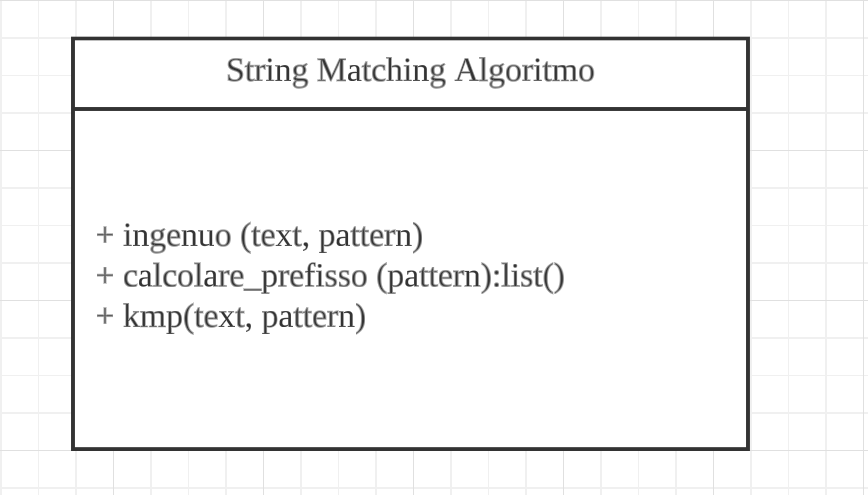
\includegraphics[width=0.8\textwidth]{Resources/string_match.png}
    \caption{Diagramma degli algoritmi di String Match}
    \label{fig:Ingenuo_Kmp_1}
\end{figure}

In più ho scritto delle funzioni semplicemente al fine di svolgere degli test. \textbf{TestGenerator} è utile per la generazione di infografiche utili per vedere la funzione che si evolve nel tempo dei due metodi che andrò ad analizzare.

\begin{figure}[H]
    \centering
    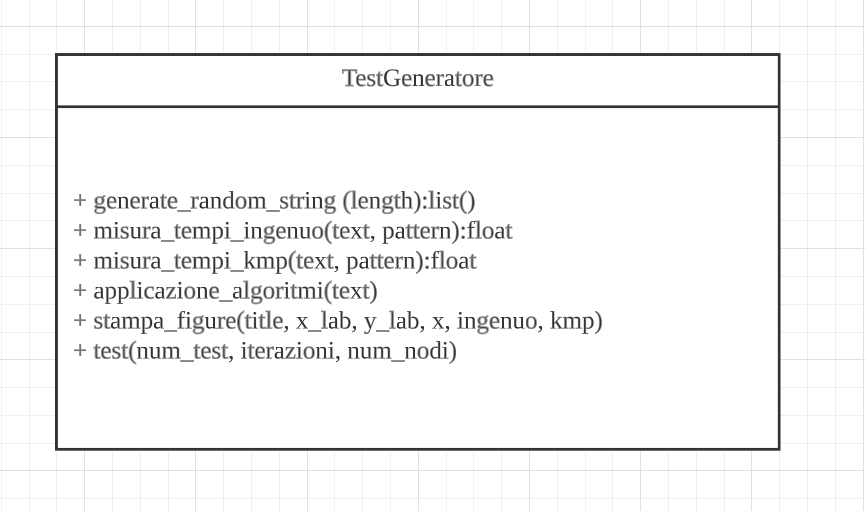
\includegraphics[width=0.7\textwidth]{Resources/testgeneratore.png}
    \caption{Diagramma di TestGenerator}
    \label{fig:TestGenerator_1}
\end{figure}

\subsection{Analisi delle scelte implementative}
\label{sec:AnalisiScelteImplementative_1}
Partendo dalla funzione \textbf{Ingenuo}, qui la scelta implementativa è di utilizzare un generatore \textbf{yield}, che un normale return, per restituire le posizioni in cui il pattern è stato trovato. Questa scelta consente di risparmiare memoria, poiché le posizioni non vengono generate tutte contemporaneamente ma solo quando necessario. Analogamente anche la funzione kmp usa \textbf{yield}, questo approccio consente una gestione efficiente delle posizioni in cui il pattern è stato trovato. In più questo algoritmo sfrutta la funzione di prefisso calcolata dalla funzione \textbf{calcolareprefisso} per saltare direttamente alle posizioni potenzialmente corrispondenti nella stringa di testo.Per calcolare la funzione di prefisso, la funzione utilizza un array \textbf{prefix} di lunghezza uguale a quella del pattern. Ogni elemento in questo array rappresenta la lunghezza del prefisso più lungo che è anche un suffisso per la sottostringa del pattern fino a quella posizione.
 
\subsection{Descrizione dei metodi implementati}
\label{sec:DescrizioneMetodiImplementati_1}
In questa parte descriverò le funzionalità di ogni metodo di cui finora abbiamo parlato.

\begin{itemize}
    \item \textbf{String Match Algoritmo}
    \begin{itemize}
        \item \textbf{ingenuo(text, pattern)}:L'algoritmo ingenuo esamina tutte le posizioni del testo alla ricerca di una corrispondenza esatta del pattern. Ogni volta che viene trovata una corrispondenza, l'indice in cui inizia la corrispondenza viene restituito tramite un generatore.
        \item \textbf{calcolarePrefisso(pattern)}: La funzione calcolarePrefisso calcola la funzione di prefisso per il pattern fornito. Questa funzione calcola il più lungo prefisso proprio che è anche un suffisso per ogni sottostringa del pattern. I risultati vengono restituiti come una lista di interi.
        \item \textbf{kmp(text, pattern)}:L'algoritmo kmp utilizza la funzione di prefisso calcolata dalla funzione calcolareprefisso per eseguire una ricerca efficiente del pattern nel testo. Ogni volta che viene trovata una corrispondenza, l'indice in cui inizia la corrispondenza viene restituito tramite un generatore.
    \end{itemize}
    \item \textbf{TestGenerator}
    \begin{itemize}
        \item \textbf{generateRandomString(length)}:Questo metodo genera una stringa casuale di una data lunghezza utilizzando lettere maiuscole, minuscole e cifre. Restituisce la stringa generata.
        \item \textbf{misuraTempiIngenuo(text, pattern)}:Questo metodo misura il tempo impiegato per eseguire l'algoritmo di ricerca ingenuo sul testo e restituisce il tempo trascorso.
        \item \textbf{misuraTempiKmp(text, pattern)}:Questo metodo misura il tempo impiegato per eseguire l'algoritmo KMP sul testo e restituisce il tempo trascorso.
        \item \textbf{applicazioneAlgoritmo(text, pattern)}:Questo metodo chiama misuraTempiIngenuo e misuraTempiKmp per misurare i tempi impiegati dagli algoritmi ingenuo e KMP e restituisce i risultati in una tupla.
        \item \textbf{stampaFigure(title, xlab, ylab, x, naive, kmp)}:Questo metodo crea un grafico con il titolo e le etichette specificate e lo restituisce come oggetto figura Matplotlib.
        \item \textbf{test(numtest, iterazioni, lunghezzatesto, lunghezzapattern)}:Questo metodo esegue una serie di test nei quali genera stringhe casuali di lunghezze variabili, quindi applica gli algoritmi ingenuo e KMP per misurare i tempi impiegati. I risultati vengono raccolti e analizzati per determinare quale algoritmo è più efficiente in base ai tempi medi di esecuzione. Infine, crea un grafico dei tempi di esecuzione.
    \end{itemize}
\end{itemize}

\newpage
\section{Descrizione degli esperimenti condotti e analisi dei risultati sperimentali}

\subsection{Dati utilizzati}
\label{sec:DatiUtilizzati_1}
L'obiettivo di questo esperimento era misurare i tempi di esecuzione degli algoritmi di ricerca di stringhe \textbf{Ingenuo} e \textbf{KMP} su stringhe casuali di lunghezza variabile. Sono stati condotti test in cui sono state variate la lunghezza del testo e del pattern per valutare le prestazioni relative di questi algoritmi.

Abbiamo suddiviso l'esperimento in parti, ciascuna con configurazioni specifiche per la lunghezza del testo e del pattern:

\begin{itemize}
    \item Testo di lunghezza \textbf{10} e Pattern di lunghezza \textbf{2}
    \item Testo di lunghezza maggiore di \textbf{100} e Pattern di lunghezza \textbf{2}
\end{itemize}

In ogni parte, abbiamo generato automaticamente stringhe casuali per il testo e il pattern, vedi in figura \ref{fig:randomStringhe}. Le stringhe casuali sono state create con caratteri alfanumerici casuali. Il testo ha avuto una variazione nella lunghezza, mentre il pattern è rimasto costante a 2 caratteri.

\begin{figure}[H]
    \centering
    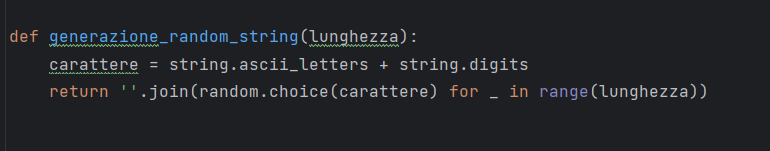
\includegraphics[width=0.6\textwidth]{Resources/generazionerandomstring.png}
    \caption{Come vengono generati le stringhe}
    \label{fig:randomStringhe}
\end{figure}

Abbiamo utilizzato le funzioni \textbf{Ingenuo} e \textbf{KMP} per cercare il pattern all'interno del testo. In ciascun test, abbiamo registrato il tempo impiegato da ciascun algoritmo per completare la ricerca.

\subsection{Misurazione}
\label{sec:Misurazioni_1}
I metodi di calcolo dei tempi sono nei metodi \textbf{misuraTempiIngenuo} e \textbf{misuraTempiKmp}. Innanzitutto dobbiamo prendere il tempo prima dell'esecuzione del metodo e quello dopo la sua esecuzione (esempio in figura \ref{fig:codicePrendereTempo}). 

\begin{figure}[H]
    \centering
    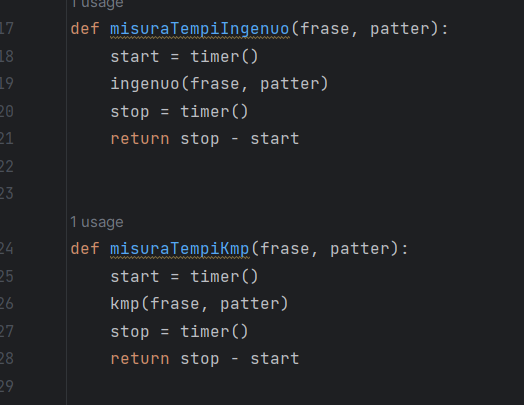
\includegraphics[width=0.6\textwidth]{Resources/tempi.png}
    \caption{Come vengono presi i tempi nel codice}
    \label{fig:codicePrendereTempo}
\end{figure}

Questo fa si che per calcolare i tempi si possano usare:

\begin{equation}
    timeArray[x+1]=(end-start)+timeArray[x];
    \label{eqn:timeArray1}
\end{equation}

che calcola sempre il tempo che ci vuole ogni qualvolta si compie un iterazione che aumenta la lunghezza delle stringhe.

\subsection{Risultati sperimentali e commenti analitici}
\label{sec:RisultatiSperimentaliCommentiAnalitici_1}
\subsection{Testo di lunghezza 10 e Pattern di lunghezza 2}
Durante gli esperimenti, abbiamo osservato risultati interessanti e variazioni nelle prestazioni degli algoritmi. Notiamo come in figura \ref{fig:lunghezza10} in alcune circostanze, l'algoritmo \textbf{Ingenuo} ha dimostrato di essere più veloce dell'algoritmo \textbf{KMP}.Questo è stato particolarmente evidente quando sia il testo che il pattern avevano lunghezze relativamente brevi. In questo caso nei testi con lunghezze da 10 fino a 20. Anche nella figura \ref{fig:lenght10_1} l'algoritmo \textbf{Ingenuo} ha mostrato la sua efficienza rispetta all'algoritmo \textbf{KMP} per testi con lunghezza 40.
\begin{figure}[H]
    \centering
    \begin{subfigure}[b]{0.49\textwidth}
        \centering
        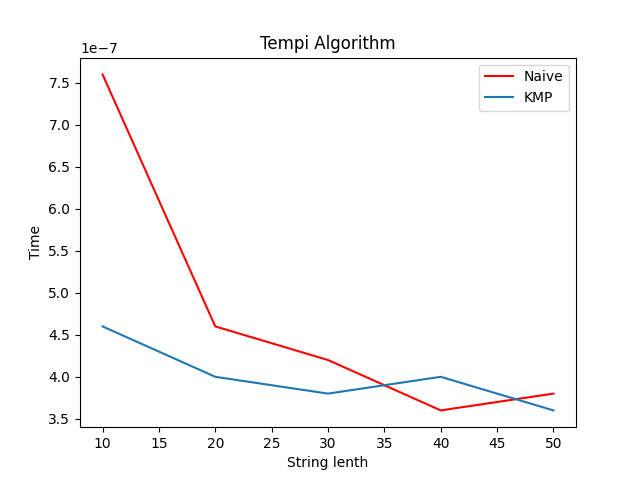
\includegraphics[width=\textwidth]{Resources/lenght10_1.png}
        \caption{Testo di lunghezza 10}
        \label{fig:lenght10_1}
    \end{subfigure}
    \hfill
    \begin{subfigure}[b]{0.49\textwidth}
        \centering
        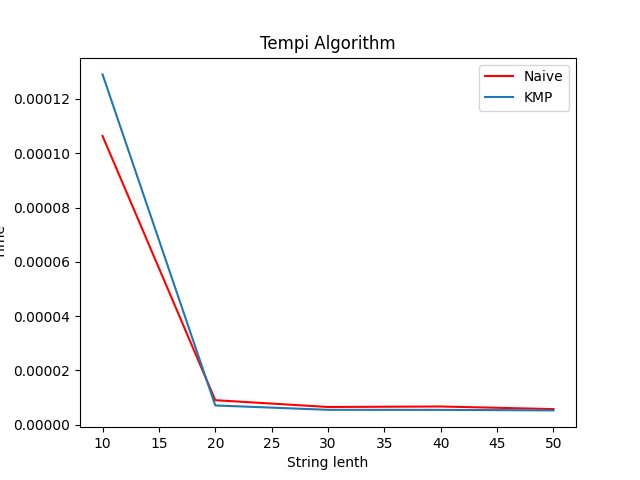
\includegraphics[width=\textwidth]{Resources/lunghezza10.png}
        \caption{Testo di lunghezza 10}
        \label{fig:lunghezza10}
    \end{subfigure}
    \caption{Testo di lunghezza 10 e pattern 2}
    \label{fig:lunghezza10_12}
\end{figure}

\subsection{Testo di lunghezza maggiore di 100 e pattern 2}
In questi esperimenti, abbiamo condotto ricerche di pattern di 2 caratteri all'interno di un testo lungo maggiore di 100 caratteri. In ogni test, abbiamo registrato i tempi di esecuzione degli algoritmi \textbf{Ingenuo} e \textbf{KMP}. In tutti i casi, l'algoritmo \textbf{KMP} è emerso come la scelta più efficiente rispetto all'approccio \textbf{Ingenuo}. In tutte le prove effettuate  l'algoritmo \textbf{KMP} ha dimostrato una performance costantemente superiore rispetto all'algoritmo \textbf{Ingenuo}. Questa costanza nella superiorità di \textbf{KMP} sottolinea la sua efficienza intrinseca nella ricerca di pattern all'interno di stringhe.La costanza dei risultati suggerisce che la lunghezza del testo non ha un impatto significativo sulle prestazioni relative degli algoritmi in questo particolare contesto, come in figura \ref{fig:test_1000}. Anche con un testo relativamente lungo, \textbf{KMP} riesce a mantenere un vantaggio distintivo.Questi risultati riflettono la complessità computazionale dell'algoritmo \textbf{KMP}. Grazie alla tavola di fallimento e all'approccio basato su pre-elaborazione, \textbf{KMP} è in grado di evitare ricerche inutili e ridurre notevolmente il tempo di esecuzione, anche con pattern di piccole dimensioni, in figura \ref{fig:test_100}.
\begin{figure}[H]
    \centering
    \begin{subfigure}[b]{0.49\textwidth}
        \centering
        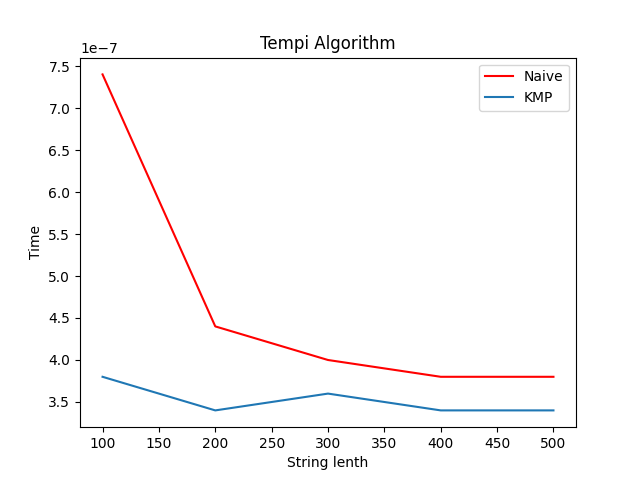
\includegraphics[width=\textwidth]{Resources/lenght100_2.png}
        \caption{Testo lungo 100}
        \label{fig:lenght100_1}
    \end{subfigure}
    \hfill
    \begin{subfigure}[b]{0.49\textwidth}
        \centering
        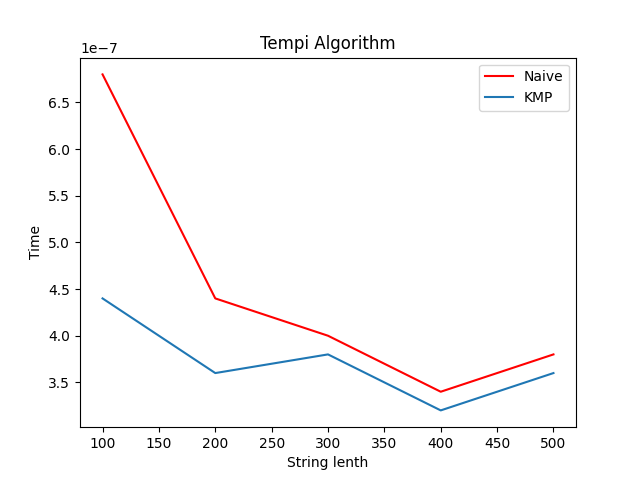
\includegraphics[width=\textwidth]{Resources/lenght100_3.png}
        \caption{Testo lungo 100}
        \label{fig:lenght100_2}
    \end{subfigure}
    \caption{Test svolti con testo lungo 100 e pattern 2}
    \label{fig:test_100}
\end{figure}

\begin{figure}[H]
    \centering
    \begin{subfigure}[b]{0.49\textwidth}
        \centering
        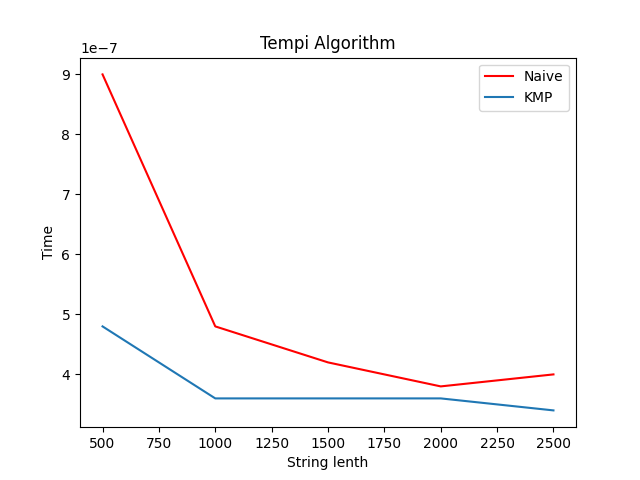
\includegraphics[width=\textwidth]{Resources/lenght500_1.png}
        \caption{Testo lungo 500}
        \label{fig:lenght500_1}
    \end{subfigure}
    \hfill
    \begin{subfigure}[b]{0.49\textwidth}
        \centering
        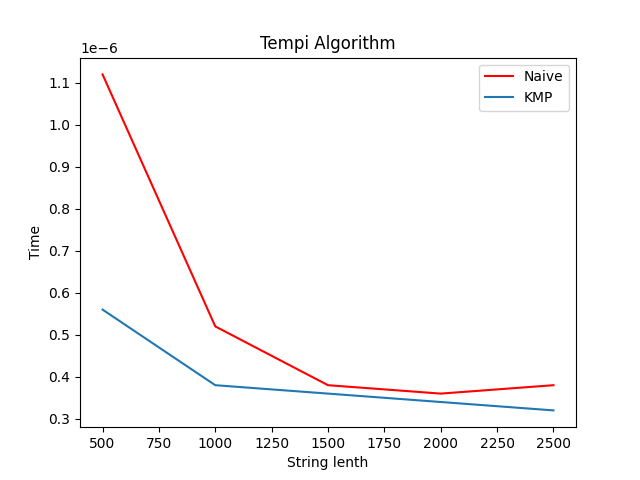
\includegraphics[width=\textwidth]{Resources/lenght500_2.png}
        \caption{Testo lungo 500}
        \label{fig:lenght500_2}
    \end{subfigure}
    \caption{Test svolti con testo lungo 500 e pattern 2}
    \label{fig:test_500}
\end{figure}

\begin{figure}[H]
    \centering
    \begin{subfigure}[b]{0.49\textwidth}
        \centering
        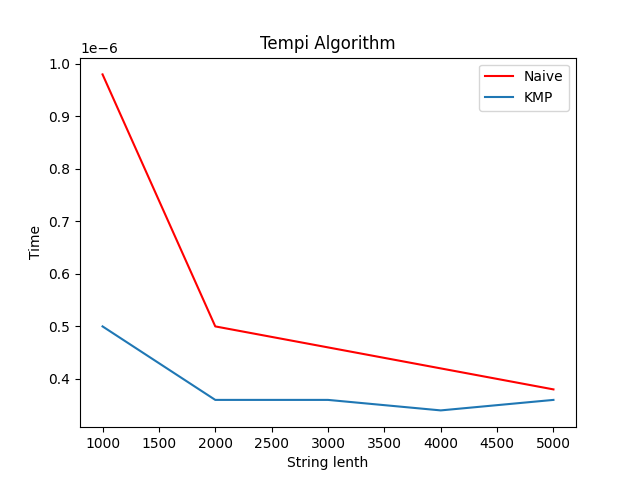
\includegraphics[width=\textwidth]{Resources/lenght1000_1.png}
        \caption{Testo lungo 1000}
        \label{fig:lenght1000_1}
    \end{subfigure}
    \hfill
    \begin{subfigure}[b]{0.49\textwidth}
        \centering
        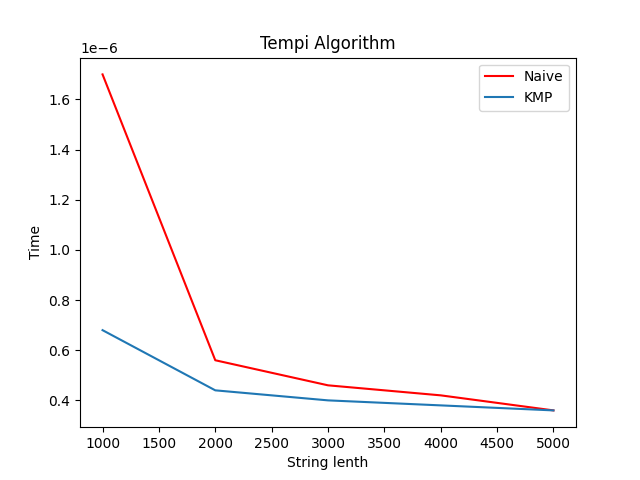
\includegraphics[width=\textwidth]{Resources/lenght1000_2.png}
        \caption{Testo lungo 1000}
        \label{fig:lenght1000_2}
    \end{subfigure}
    \caption{Test svolti con testo lungo 1000 e pattern 2}
    \label{fig:test_1000}
\end{figure}

\subsection{Conclusione Generale}
In base all'analisi approfondita degli esperimenti condotti, è evidente che gli algoritmi di ricerca di stringhe \textbf{Ingenuo} e \textbf{KMP} presentano differenze significative nelle loro prestazioni e complessità computazionale. Dai risultati ottenuti, è chiaro che \textbf{KMP} si è dimostrato costantemente più efficiente dell'approccio \textbf{Ingenuo} nella maggior parte delle condizioni.

L'efficienza di \textbf{KMP} deriva dalla sua complessità computazionale ottimizzata, che gli consente di evitare ricerche inutili nel testo. Questa efficienza è particolarmente evidente quando il pattern è relativamente breve rispetto al testo o quando entrambi sono di grandi dimensioni.

La scelta tra gli algoritmi \textbf{Ingenuo} e \textbf{KMP} dipende dalle specifiche esigenze del problema. Se la ricerca di stringhe è un'operazione frequente o coinvolge dati di grandi dimensioni, \textbf{KMP} si presenta come la scelta più logica grazie alla sua efficienza intrinseca.

In conclusione, questo studio ha evidenziato l'importanza di selezionare l'algoritmo di ricerca di stringhe più appropriato in base alle dimensioni dei dati e alla complessità del pattern. La comprensione delle complessità computazionali e delle prestazioni relative di questi algoritmi è essenziale per prendere decisioni informate in situazioni reali.
\begin{thebibliography}{9}
\bibitem{algLib}
Thomas H. Cormen, Charles E. Leiserson, Ronald L. Rivest, Clifford Stein (2009) Introduzione agli algoritmi e strutture dati Terza edizione, McGraw Hill.

\end{thebibliography}

\end{document}
